\documentclass[12pt]{article}

\usepackage[dvips,letterpaper,margin=0.75in,bottom=0.75in]{geometry}
\usepackage{cite}
\usepackage{slashed}
\usepackage{graphicx}
\usepackage{mathtools}
\usepackage{amsmath}
\usepackage{amssymb}
\usepackage{braket}
%\usepackage[american,fulldiode]{circuitikz}
\usepackage{tikz}
\begin{document}

\title{PHY 130B \\ Lecture Notes G: \\
Introduction to Groups, Symmetries, and Lie Algebras\\}
\author{Michael Mulhearn}

\maketitle

\newcounter{exercise}
\setcounter{exercise}{0}

\newcommand{\exercise}{
\stepcounter{exercise}
\noindent
{\bf Exercise G.\theexercise:}
}

\noindent
{\it These notes are largely based on Chapters 4 and 5 of Jeevanjee's
  excellent text ``An Introduction to Tensors and Group Theory for
  Physicists'' which I highly recommend working through carefully if
  you enjoy the small taste presented here.  The online version is
  available free through the UC Davis library!}

\section{Groups and Symmetry}

\noindent
A \textbf{group} is a set $G$ with an operation $\cdot$ which satistifies:
\begin{itemize}
  \item \textbf{Closure}:  for all $g, h \in G$  
    \begin{equation*}
      g \, \cdot \, h \quad \in G 
    \end{equation*}

  \item \textbf{Associativity}:  for all $g, h, k \in G$  
    \begin{equation*}
      g \cdot (h \cdot k) \quad = \quad (g \cdot h) \cdot k
    \end{equation*}

  \item \textbf{Existence of identity}: There exists $e \in G$ such that for all $g \in G$:
    \begin{equation*}
      g \cdot e \quad = \quad e \cdot g \quad = \quad g 
    \end{equation*}

  \item \textbf{Existence of inverses}: For any $g \in G$, there exists $h \in G$ such that
    \begin{equation*}
      g \cdot h \quad = \quad h \cdot g \quad = \quad e
    \end{equation*}
\end{itemize}
Note that 
\begin{itemize}
  \item Commutativity is \emph{not} required (i.e., $g \cdot h \neq h \cdot g$ in general).
  \item The operation $\cdot$ is abstract.  it need not be multiplication in the conventional sense.  We sometimes use $\odot$ when we want to emphasize it is abstract mutiplication.
  \item In concrete cases, the operation is often composition.
\end{itemize}
There are several important properties of groups that follow directly from the axioms:
\begin{itemize}

\item {\bf The identity is unique:} Suppose $e$ and $f$ are both identities. Then:
\begin{align*}
  e &= e \cdot f \quad & (f \text{ is identity}) \\
    &= f & (e \text{ is identity}) \\
\end{align*}
\item {\bf Inverses are unique: } Suppose both $h$ and $k$ are inverses of $g$ so that:
$$ g \cdot h = h \cdot g = e$$
and  
$$ g \cdot k = k \cdot g = e$$
So then:
\begin{align*}
  gh &= gk \\
  hgh &= hgk \\
  eh &= ek \\
  h &= k \\
\end{align*}
We denote the unique inverse to $g$ as $g^{-1}$.
\item {\bf Right inverses are inverses: } Suppose that $h$ is a right inverge to $g$:
$$ gh \quad = e$$
  Then we have:
\begin{align*}
g^{-1} g h &= g^{-1} e \\
e h &= g^{-1} e \\
  h &= g^{-1} \\
\end{align*}  
A similar result holds for left inverses.  So any right or left inverse is the unique inverse $g^{-1}$. 
\end{itemize}

\subsection*{Example:  The Additive Group of Real Numbers}

Let $x,\, y \in \mathbb{R}$, with operation $x \odot y := x + y$.  We
confirm the axioms are satisfied:\\[10pt]
\textbf{Closure:}
\begin{equation*}
  x \odot y = x + y \in \mathbb{R} \quad \checkmark
\end{equation*}
\textbf{Associativity:}
\begin{equation*}
  x \odot (y \odot z) = x + (y + z)
  = (x + y) + z = (x \odot y) \odot z \quad \checkmark
\end{equation*}
\textbf{Identity:} $e = 0 \in \mathbb{R}$,
\begin{equation*}
  x \odot e = x + 0 = x \quad \checkmark
\end{equation*}
\textbf{Inverses:} $x^{-1} = -x \in \mathbb{R}$,
\begin{equation*}
  x \odot x^{-1} = x + (-x) = 0 = e \quad \checkmark
\end{equation*}

\subsection*{Example: The General Linear Group $GL(V)$}

The General Linear Group $GL(V)$ is the set of all {\bf invertible} linear operators:
$$T: V \to V$$
on a vector space $V$ with group operation being composition:
\begin{equation*}
  (T \cdot U)(x) \equiv T(U(x))
\end{equation*}
for $T,U \in GL(V)$.  Note that invertible implies that any
$T \in GL(V)$ is one-to-one and onto.  We confirm the axioms are
satisfied:\\[10pt]
\textbf{Closure:} (TU) is linear:
\begin{align*}
  (TU)(\alpha x + \beta y)
  &= T \bigl( U(\alpha x + \beta y) \bigr)\\
  &= T \bigl( \alpha U(x) + \beta U(y) \bigr) \\
  &= \alpha\, T\bigl(U(x)\bigl) + \beta\, T\bigl(U(y)\bigl) \\
  &= \alpha\, (TU) (x) + \beta\, (TU) (y) \quad \checkmark \\
\end{align*}
and (TU) in invertible because:
$$(TU)^{-1} = U^{-1} \, T^{-1}$$
works and we show below that the inverses $U^{-1}$ and $T^{-1}$ are also in GL(V).\\[5pt]
\textbf{Associativity:}
\begin{align*}
  \bigl(T(UV)\bigr)(x) &= T\!\bigl((UV)(x)\bigr)
  = \Bigl(T\bigl(U(V(x)\bigr)\Bigr) \\
   &= \bigl((TU)V\bigr)(x) \quad \checkmark
\end{align*}
\textbf{Identity:} For the identity operator $I(x) = x$:
\begin{align*}
  (TI)(x) &= T(I(x)) = T(x) \\
  (IT)(x) &= I(T(x)) = T(x) \quad \checkmark
\end{align*}
\textbf{Inverses:} For $T \in GL(V)$ then $T^{-1}$ exists by
definition, but we must show it is linear and invertible and so also
in $GL(V)$.  For any $a,b \in V$ there exists $x,y \in V$ such that:
$$a = T(x) \qquad b = T(y)$$
because $T$ is onto.  Then:
\begin{align*}
  T^{-1}(\alpha a + \beta b) \quad &= \quad T^{-1}(\alpha T(x) + \beta T(y))\\
  &= \quad T^{-1}(T(\alpha x + \beta y)) \qquad \star \\
  &= \quad \alpha x + \beta y \\
  &= \quad \alpha T^{-1}(a) + \beta T^{-1}(b) \quad \checkmark \\
\end{align*}
$T^{-1}$ is invertible because it has inverse $T$.

\subsection*{Subgroups}

A subset $H$ of $G$ called a \textbf{subgroup} if $H$ is itself a
group (using the same operation as the group $G$!)  We write:
$$H \subseteq G$$

\noindent
Some examples of subgroups:
\begin{itemize}
  \item The set ${e}$ containing only the identity is a subgroup of
    every group.  
  \item The integers $\mathbb{Z}$ are a subgroup of the additive group of real numbers $(\mathbb{R}, +)$:\\[5pt]
    \textbf{Closure:} $n + m  \in Z$ if $n,m \in Z$ \\
    \textbf{Identity:} $e = 0 \in Z$ \\
    \textbf{Inverses:} Each $n \in Z$ has inverse $-n \in Z$ 
\end{itemize}    
Note that we need not verify the associative axiom for any subgroup, since the elents of the subgroup are elements of the group, and so the axiom holds.


\subsection*{Symmetry}

Groups are the natural mathematical framework for describing symmetry.
Suppose $V$ is a vector space with an NDHF denoted:
$$(\cdot \mid \cdot)$$
The isometries of $V$, denoted $\mathrm{Isom}(V)$, are the subgroup of $GL(V)$
that preserve the NDHF.  For $T \in \mathrm{Isom}(V)$:
$$(T(u) \mid T(v)) = (u \mid v)$$
We verify the the axioms hold:\\
\textbf{Closure:}
\begin{equation*}
  \bigl((TU)(v) \mid (TU)(u)\bigr)
  = \bigl(T(U(v)) \mid T(U(u))\bigr)
  = \bigl(U(v) \mid U(u)\bigr)
  = (v \mid u) \quad \checkmark
\end{equation*}
\textbf{Identity:}
\begin{equation*}
  \bigl(I(v) \mid I(u)\bigr) = (v \mid u) \quad \checkmark
\end{equation*}
\textbf{Inverses:}
\begin{equation*}
  \bigl(T^{-1}(v) \mid T^{-1}(u)\bigr)
  = \bigl(T(T^{-1}(v)) \mid T(T^{-1}(u))\bigr)
  = (v \mid u) \quad \checkmark
\end{equation*}

\section{Homomorphisms and Isomorphisms}

For groups $G$ and $H$, a \textbf{homomorphism} $\phi: G \to H$ satisfies:
\begin{equation*}
  \phi(g \cdot h) = \phi(g) \cdot \phi(h)
\end{equation*}
for all $g,h \in G$.  You will show in the exercises that:
\begin{itemize}
\item A homomophism maps the identity to the identity:
  \begin{equation}
  \label{eqn:maps-identities}
  \phi(e_G) = e_H
\end{equation}
where $e_G$ is the identity in $G$ and $e_H$ is the indentity in $H$.
\item A homomophism maps inverses to inverses:
\begin{equation}
  \label{eqn:maps-inverses}
  \phi(g^{-1}) = \bigl(\phi(g)\bigr)^{-1}
\end{equation}
\end{itemize}
If $\phi$ is one-to-one and onto, we call it an \textbf{isomorphism} and write $G \cong H$.\\[5pt]

\exercise (*) Verify Equations~\ref{eqn:maps-identities} and
\ref{eqn:maps-inverses}. $\quad \square$\\[5pt]

\exercise For any groups $G$ and $H$, show that the map
$$\phi(g) = e$$
for all $g \in G$, where $e$ is the identity in $H$, is a homomorphism.
$\quad \square$\\[5pt]

\exercise Show that the additive group of real numbers is isomorphic to the multiplicative group of positive real numbers via the isomorphism:
$$\phi: (\mathbb{R}, +) \to (\mathbb{R}^+,\times)$$
with:
$$\phi(x) = \exp(x) \quad \square$$\\[5pt]

\subsection*{Matrix Represenation of Linear Operators}

Since the beginning of this course we have been associating tensors
$T$ with their matrix representation in a particular basis.  We can
now state this relation more precisely.  For a vector space $V$ of
over the complex numbers, with finite dimension $n$, there is an
isomorphism between the general linear group $GL(V)$ and the
invertible $n \times n$ complex matrices, $GL(n, \mathbb(C))$ given by:
$$T \mapsto [T]_{B}$$
for $T \in GL(V)$.  We'll prove this in three steps:
\begin{enumerate}
  \item Show $[TU] = [T][U]$ (homomorphism, i.e.\ $GL(V) \to GL(n,\mathbb{C})$ is a homomorphism)
  \item Show $[T] \in GL(n,\mathbb{C})$ (onto)
  \item Show it is one-to-one $\implies$ isomorphism \checkmark
\end{enumerate}
\textbf{Step 1:} We'll show that:
$$[TU] = [T][U]$$
For clearer notation, define:
$$w = U(v)$$
where $U$ is a linear operator, equivalently represented by a (1,1) tensor, so that:
$$w^j = U^j_k \, v^k$$
Also defining:
$$x = (TU)(v)$$
which has matrix representation:
$$[x] = [TU][v]$$
but can also be written as:
$$x = T\bigl(U(v)\bigr) = T(w)$$
and so:
$$x^i = T^i{}_j w^j = T^i{}_j\,U^j{}_k\,w^k$$
which has matrix representation:
$$[x] = [T][U][v]$$
So
$$[TU][v] = [T][U][v]$$
and as $v$ is arbitrary:
$$[TU]=[T][U]$$
So we have shown that $T \mapsto [T]_\mathcal{B}$ is a homomorphism.\\[5pt]

\noindent
\textbf{Step 2:} We'll show that the homomorphism is onto.  For any matrix $M \in GL(n,\mathbb{C})$, define a linear operator $T$ by its action on a vector $v$ via the compoments of $M$:
\begin{equation*}
  T(v) = M^i{}_j\, v^j\, e_i
\end{equation*}
Then by construction $[T] = M$, so the map is onto $GL(n,\mathbb{C})$.\\[5pt]

\noindent
\textbf{Step 3:} We'll show that the homomorphism is one-to-one.  Suppose that
$$[T]=[S]$$
so
$$T^i{}_j = S^i{}_j$$
or equivalently:
$$T(e_i) = S(e_i)$$
So:
$$T(v) = v^i\,T(e_i) = v^i S(e_i) = S(v)$$
and hence:
$$T = S$$
thus the homomorphism is one-to-one.

Together, these results show that the map:
$$T \mapsto  [T]_\mathcal{B}$$
is an isomorphism.

\subsection*{Isometry Groups}

Suppose we have a vector space $V$ with an NDHF. We showed previously
that the isometry group of $V$, denoted $\mathrm{Isom(V)}$, are a
subgroup of the general linear group $GL(V)$ with the defining
property
$$\bigl( T(u) \mid T(v) \bigr) = (u \mid v)$$ for all $T \in
\mathrm{Isom}(V)$ and $u,v \in V$.  We also just showed that $GL(V)$
is isomorphic to $n \times n$ invertible matrices $GL(n,\mathbb{C})$.
Therefore:\\
\medskip
\noindent\fbox{\parbox{0.9\textwidth}{
Isometries can be faithfully represented by a subset of invertible $n \times n$ matrices.
}}\\
or equivalently:
$$\mathrm{Isom}(V) \subseteq GL(n,\mathbb{C})$$

\subsection*{Rotations and Reflections}

For a real vector space $V$ with Euclidean metric,
$$(x \mid y) = [x]^T [y]$$
the isometries $A$ satisfy
$$(Ax \mid Ay) = (x \mid y)$$
and so:
\begin{align*}
  [A\,x]^T[A\,y] &= [x]^T[y] \\
  [x]^T [A]^T [A]\,[y] &= [x]^T[y]
\end{align*}
and so
\begin{equation}
  \label{eqn:othogonal-group}  
  [A]^T [A] = I
\end{equation}
which is the defining property of the Orthogonal group:
\begin{equation*}
  O(n) = \bigl\{R \in GL(n,\mathbb{R}) \mid R^T R = I\bigr\}
\end{equation*}
Note that:
\begin{equation*}
  \det(R^T R) = \bigl(\det R\bigr)^2 = 1 \implies \det(R) = \pm 1
\end{equation*}
We define the Special Orthogonal group SO(n) as the elements of O(n) with determinant 1.
\begin{equation*}
  SO(n) = \bigl\{R \in O(n) \mid \det(R) = +1 \bigr\}
\end{equation*}
\\[3pt]

\exercise (*) The isomorphism between $GL(V)$ and $GL(n,\mathbb{C})$
insures that
$$O(n) \subseteq GL(n,\mathbb{R})$$
because
$$\mathrm{Isom(V)} \subseteq GL(V)$$
but show explicitly that Equation~\ref{eqn:othogonal-group} defines a group.
$\quad \square$\\[5pt]

\exercise (*) Show that $SO(n)$ is a subgroup of $O(n)$.  Hint: use:
$$\det(AB) = \det(A) \det(B) \quad \square$$\\[5pt]

\noindent
In the exercises that follow, you'll show that $SO(2)$ contains only proper rotations of form:
\begin{equation}
\label{eqn:proper-rotation}
R(\theta) = \begin{pmatrix} \cos\theta & -\sin\theta \\ \sin\theta & \cos\theta \end{pmatrix},
\end{equation}
but O(2) includes reflections (or parity inversion)
\begin{equation}
\label{eqn:parity-inversion}
P = \begin{pmatrix} 1 & 0 \\ 0 & -1 \end{pmatrix},
\end{equation}
and improper rotations of form $P R(\theta)$.\\[5pt]

\exercise (*) Show that:
$$SO(2) = \bigl\{R(\theta) \mid \theta \in \mathbb{R} \bigr\}$$
that is SO(2) contains only (proper) rotations of the form Equation~\ref{eqn:proper-rotation}$\quad \square$\\[5pt]

\exercise (*) Show that:
$$R(\theta)^T = R(-\theta)$$
This presents a nice way to think about why
$$R^T R = I$$
for rotations.

\exercise (*) Calculate the general form of an improper rotation from:
$$P R(\theta)$$
and compute it's determinant.

\exercise  Show that:
$$O(2) = \bigl\{R(\theta) \mid \theta \in \mathbb{R}\bigr\}
\cup \bigl\{P\,R(\theta) \mid \theta \in \mathbb{R}\bigr\} \quad \square$$

\subsection*{Unitary Group}

For a finite-dimensional complex inner product space, with:
$$\braket{\phi \mid \psi} = [\phi]^\dagger [\psi]$$
the isometries satisfy
$$\braket{A\phi \mid A\psi} = \braket{\phi \mid \psi}$$
and so
\begin{align*}
  [A\phi]^\dagger [A\psi] &= [\phi]^\dagger [A]^\dagger [A]\,[\psi] \\
  [A]^\dagger [A] &= I
\end{align*}

We define the Unitary group as:
\begin{equation*}
  U(n) = \bigl\{U \in GL(n,\mathbb{C}) \mid U^\dagger U = I\bigr\}
\end{equation*}
Note that
\begin{equation*}
  \det(U^\dagger U) = \det(I)
  \implies \overline{\det(U)}\cdot\det(U) = 1
  \implies |\det(U)|^2 = 1
  \implies |\det(U)| = 1
\end{equation*}
We define the Special Unitary group as:
\begin{equation*}
  SU(n) = \bigl\{U \in U(n) \mid \det(U) = 1\bigr\}
\end{equation*}

\noindent
\textbf{Claim:} For an orthonormal basis $B$:
\begin{equation*}
  [U^\dagger]_B = [U]^\dagger_B
\end{equation*}
We will occassionally need this, but we won't prove it here.  See problem 2.7 in Jeevanjee for how to prove it.\\[5pt]

\exercise (*) Show that:
$$U(1) = \bigl\{e^{i\theta} \mid \theta \in \mathbb{R} \bigr\}$$
and
$$SU(1) = {1} \quad \square $$

\section{SU(2) and SO(3)}

\subsection*{The Group SO(3)}

We have already seen that $SO(3)$ consists of the real $3\times 3$ matrices
satisfying $R^T R = I$ with $\det(R) = +1$.  These are precisely the proper
rotations of $\mathbb{R}^3$.  Any element of $SO(3)$ can be written as a
rotation about some axis, and the group is parameterized by \textbf{3
parameters} (e.g.\ three Euler angles, or an axis direction plus an angle).

Rotations about the three coordinate axes are given by:
\begin{equation*}
  R_x(\theta) = \begin{pmatrix} 1 & 0 & 0 \\ 0 & \cos\theta & -\sin\theta \\ 0 & \sin\theta & \cos\theta \end{pmatrix}, \quad
  R_y(\theta) = \begin{pmatrix} \cos\theta & 0 & \sin\theta \\ 0 & 1 & 0 \\ -\sin\theta & 0 & \cos\theta \end{pmatrix}, \quad
  R_z(\theta) = \begin{pmatrix} \cos\theta & -\sin\theta & 0 \\ \sin\theta & \cos\theta & 0 \\ 0 & 0 & 1 \end{pmatrix}.
\end{equation*}
A general rotation $R(\psi,\theta,\phi) \in SO(3)$ can be expressed in terms
of these, using 3 parameters.

\subsection*{The Group SU(2)}

$SU(2)$ is the group of $2\times 2$ complex unitary matrices with determinant
one:
\begin{equation*}
  SU(2) = \bigl\{ A \in GL(2,\mathbb{C}) \mid A^\dagger A = I,\; \det A = 1 \bigr\}.
\end{equation*}
A general element has the form:
\begin{equation*}
  A = \begin{pmatrix} \alpha & \beta \\ -\bar\beta & \bar\alpha \end{pmatrix}, \qquad |\alpha|^2 + |\beta|^2 = 1.
\end{equation*}
\textbf{Parameter count:} $A \in GL(2,\mathbb{C})$ has $2\times 2 = 4$ complex
entries, giving 8 real parameters.  The unitary constraint $A^\dagger A = I$
imposes 4 real constraints, leaving 4 parameters; the determinant condition
imposes 1 more, leaving \textbf{3 parameters} — the same as $SO(3)$.

\exercise (*) Verify that the general form above satisfies $A^\dagger A = I$
and $\det A = 1$. $\quad\square$\\[5pt]

\subsection*{The Pauli Space $\mathcal{C}_P$}

\noindent
\textbf{Definition:} The \textbf{Pauli space} $\mathcal{C}_P$ is the real
vector space of $2\times 2$ traceless Hermitian matrices.

\noindent
\textbf{Note:} The Pauli matrices
\begin{equation*}
  \sigma_x = \begin{pmatrix}0&1\\1&0\end{pmatrix},\quad
  \sigma_y = \begin{pmatrix}0&-i\\i&0\end{pmatrix},\quad
  \sigma_z = \begin{pmatrix}1&0\\0&-1\end{pmatrix}
\end{equation*}
are a basis for $\mathcal{C}_P$, and a general element is
\begin{equation*}
  X = x\,\sigma_x + y\,\sigma_y + z\,\sigma_z = \begin{pmatrix} z & x-iy \\ x+iy & -z \end{pmatrix}, \qquad x,y,z \in \mathbb{R}.
\end{equation*}
Note that $X \in GL(\mathcal{C}_P)$ is a 2$\times$2 matrix acting on a 3-dimensional
real vector space, so $\mathcal{C}_P \cong \mathbb{R}^3$.  A key
identity is:
\begin{equation}
  \label{eqn:det-pauli}
  -\det(X) = x^2 + y^2 + z^2,
\end{equation}
so $-\det(X)$ is precisely the squared Euclidean norm of the corresponding
vector $(x,y,z) \in \mathbb{R}^3$.  \textbf{Careful:} $[X]$ is a $2\times 2$
matrix whose column vectors are \emph{not} the components of $x$; the components
$(x,y,z)$ must be read off from the matrix entries.

\exercise (*) Verify Equation~\ref{eqn:det-pauli}.  Also show that
$-\det(X) = ([x]^T[x])$, i.e.\ it equals the squared Euclidean norm.
$\quad\square$\\[5pt]

\subsection*{The Homomorphism $\rho: SU(2) \to SO(3)$}

For each $A \in SU(2)$, define a linear operator $L: \mathcal{C}_P \to \mathcal{C}_P$ by:
\begin{equation*}
  L(X) = A\,X\,A^\dagger.
\end{equation*}
We verify that $L$ maps $\mathcal{C}_P$ to itself and defines a group
homomorphism.

\noindent\textbf{Invertible:} $L^{-1}(X) = A^\dagger X A$, so $L \in GL(\mathcal{C}_P)$. \\[3pt]
\noindent\textbf{Linear:} 
\begin{equation*}
  L^{-1}(L(L(X))) = L^{-1}(\alpha X + \beta Y) = A^\dagger(\alpha X + \beta Y)A = \alpha\,A^\dagger X A + \beta\,A^\dagger Y A \quad\checkmark
\end{equation*}
\noindent\textbf{Hermitian:}
\begin{equation*}
  (AXA^\dagger)^\dagger = (A^\dagger)^\dagger X^\dagger A^\dagger = AXA^\dagger \quad\checkmark
\end{equation*}
\noindent\textbf{Traceless:}
\begin{equation*}
  \mathrm{Tr}(AXA^\dagger) = \mathrm{Tr}(X\,A^\dagger A) = \mathrm{Tr}(X) = 0 \quad\checkmark
\end{equation*}
So $L \in GL(\mathcal{C}_P)$.  Now define $\rho: SU(2) \to GL(\mathcal{C}_P) \cong GL(3,\mathbb{R})$ by $\rho(A) = L$.

\noindent\textbf{Homomorphism:} For $A, B \in SU(2)$:
\begin{equation*}
  \rho(AB)[X] = (AB)X(AB)^\dagger = A(BXB^\dagger)A^\dagger = \rho(A)\bigl(\rho(B)[X]\bigr) \quad\checkmark
\end{equation*}
\noindent\textbf{Image in $SO(3)$:} Since $\det(AXA^\dagger) = \det(X)$ (as
$\det(A)=1$), the operator $\rho(A)$ preserves $-\det(X) = x^2+y^2+z^2$,
i.e.\ it is an isometry of $\mathbb{R}^3$.  So $\rho(A) \in O(3)$.  By
continuity of the determinant and the fact that $\rho(I) = I$ has
$\det = +1$, we have $\det(\rho(A)) = +1$, so $\rho(A) \in SO(3)$.

\noindent\textbf{Onto:} The action of $L$ is just a rotation of $(x,y,z)$;
one can show (see HW) that every rotation in $SO(3)$ arises from some
$A \in SU(2)$.

\noindent\textbf{Not one-to-one:} Note that $\rho(-A)[X] = (-A)X(-A)^\dagger = AXA^\dagger = \rho(A)[X]$.
So $\rho(A) = \rho(-A)$ for every $A \in SU(2)$: the map is \textbf{2-to-1}.
We say that $SU(2)$ is the \textbf{double cover} of $SO(3)$.

\exercise (*) Show that $\rho$ is onto $SO(3)$ by showing $R_z(\theta) =
\rho(A)$ for
\begin{equation*}
  A = \begin{pmatrix} e^{i\theta/2} & 0 \\ 0 & e^{-i\theta/2} \end{pmatrix}
\end{equation*}
and finding similar $A$'s for $R_x$ and $R_y$. $\quad\square$\\[5pt]

\exercise (*) Verify that $R(\psi,\theta,\phi) = \rho(A(\psi,\theta,\phi))$
has the same 3 parameters as the general SU(2) element, and confirm that the
period of $\rho$ is $4\pi$ (i.e.\ $A$ must rotate by $4\pi$ to return to the
identity, whereas $R(\theta)$ has period $2\pi$).  This is the origin of
half-integer spin. $\quad\square$\\[5pt]

\section{Lie Groups and Lie Algebras}

\subsection*{Lie Groups}

\noindent
\textbf{Intuition:} A Lie group $G$ is a group that is also a smooth
manifold: near each element, it looks like $\mathbb{R}^n$ for some
dimension $n$.

\begin{center}
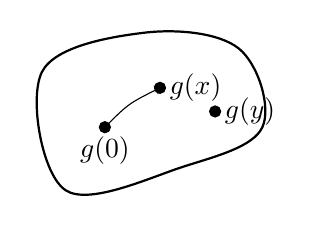
\begin{tikzpicture}
  \draw[thick] plot[smooth cycle, tension=0.6]
    coordinates {(0,0) (1.5,0.3) (2.5,0.8) (2.2,1.8) (1,2) (-0.3,1.5)};
  \filldraw (0.5,0.8) circle (2pt) node[below] {$g(0)$};
  \filldraw (1.2,1.3) circle (2pt) node[right] {$g(x)$};
  \filldraw (1.9,1.0) circle (2pt) node[right] {$g(y)$};
  \draw[->] (0.5,0.8) .. controls (0.8,1.1) .. (1.2,1.3);
\end{tikzpicture}
\end{center}

\noindent
\textbf{Pragmatic Definition:} A \textbf{matrix Lie group} $G$ is a closed
subgroup of $GL(n,\mathbb{C})$:
\begin{quote}
  \textit{If $A_n \in G$ is any sequence with $A_n \to A$, then either
  $A \in G$ or $A$ is not invertible.}
\end{quote}
\noindent\textbf{Example:} $O(n)$ is a matrix Lie group.  Put
$f(A) = A^T A$; this is a continuous function, so $f(A) = I$ defines a
closed set.  Similarly $SO(n)$, $U(n)$, $SU(n)$ are all matrix Lie groups.\\[5pt]

\noindent\textbf{Examples and their dimensions:}
\begin{itemize}
  \item $SO(2) = \{R(\theta) \mid \theta \in \mathbb{R}\}$, a \textbf{Lie
    group of dimension 1} (proper rotations of the plane, parameterized
    by one angle).
  \item $O(2)$ includes reflections, so it has two connected components
    ($\det = \pm 1$); it is technically a \textbf{Lie group of dimension 0}
    (in the sense that it is not connected, though it is still 1-dimensional
    as a manifold).
  \item $\{I, -I\} \subseteq SU(2)$: sequences converge only to $I$ or $-I$,
    so this is a \textbf{0-dimensional} closed (but not connected) Lie group.
\end{itemize}

\subsection*{Lie Algebras and Symmetry}

The key to making Lie groups tractable is to work with the tangent space at the
identity — the \textbf{Lie algebra}.

\noindent\textbf{Observation:} Suppose $G$ is a matrix Lie group with
isometries, e.g.\ $SO(n)$ or $SU(n)$.  Consider a smooth path
$U(\theta) \in G$ with $U(0) = I$.  Then:
\begin{equation*}
  U(\theta) = \exp(i\theta\, T) \approx I + i\theta\, T \quad \text{for small } \theta,
\end{equation*}
where
\begin{equation*}
  T = (-i)\,\frac{dU}{d\theta}\bigg|_{\theta=0}.
\end{equation*}
We call $T$ a \textbf{generator} of $G$.  The set of all such generators
forms the Lie algebra $\mathfrak{g}$.

\noindent
\fbox{\parbox{0.9\textwidth}{
  If $G \ni U(\theta) = \exp(i\theta T)$, then $T$ is a generator of $G$.  We call $\mathfrak{g}$ the set of generators a \textbf{symmetry} of $G$.
}}\\[8pt]

\noindent\textbf{Generators of $SO(3)$:} Taking derivatives of the rotation
matrices at $\theta=0$ and dividing by $i$:
\begin{equation*}
  L_x = (-i)\frac{dR_x}{d\theta}\bigg|_0 = \begin{pmatrix}0&0&0\\0&0&-i\\0&i&0\end{pmatrix},\quad
  L_y = \begin{pmatrix}0&0&i\\0&0&0\\-i&0&0\end{pmatrix},\quad
  L_z = \begin{pmatrix}0&-i&0\\i&0&0\\0&0&0\end{pmatrix}.
\end{equation*}
These are traceless, Hermitian (i.e.\ $L_k^\dagger = L_k$), and satisfy the
commutation relations
\begin{equation}
  \label{eqn:angular-momentum-algebra}
  [L_x, L_y] = i L_z, \qquad [L_y, L_z] = i L_x, \qquad [L_z, L_x] = i L_y.
\end{equation}

\exercise (*) Compute $[L_x, L_y]$ explicitly and verify it equals $iL_z$.
$\quad\square$\\[5pt]

\subsection*{Matrix Lie Algebras}

\noindent\textbf{Definition:} The \textbf{matrix Lie algebra} $\mathfrak{g}$
of a matrix Lie group $G$ is:
\begin{equation*}
  \mathfrak{g} = \bigl\{ X \in M_n(\mathbb{C}) \mid e^{tX} \in G \text{ for all } t \in \mathbb{R} \bigr\}.
\end{equation*}

\noindent\textbf{Theorem:} $\mathfrak{g}$ is a real vector space closed under
the \textbf{Lie bracket} $[X,Y] = XY - YX$.  That is:
\begin{enumerate}
  \item $\mathfrak{g}$ is a real vector space: if $X, Y \in \mathfrak{g}$ and
    $\lambda \in \mathbb{R}$, then $X + Y \in \mathfrak{g}$ and $\lambda X \in \mathfrak{g}$.
  \item $\mathfrak{g}$ is closed under the bracket: $[X,Y] \in \mathfrak{g}$.
  \item All elements of $\mathfrak{g}$ satisfy the \textbf{Jacobi identity}:
    \begin{equation*}
      [A,[B,C]] + [B,[C,A]] + [[C,A],B] = 0.
    \end{equation*}
\end{enumerate}

\noindent\textbf{Example:} For $G = O(n)$ with $R^TR = I$, we showed previously
that the generators satisfy $T^T = -T$ (antisymmetric real matrices), and
$\mathrm{Tr}(T) = 0$ follows automatically.  For $G = SU(n)$, the generators
are traceless Hermitian matrices.

\subsection*{The Lie Algebras of SU(2) and SO(3)}

\noindent\textbf{Theorem (Isomorphism between Lie algebras):}
If there is a continuous homomorphism $\phi: G \to H$ between Lie groups, it
induces a Lie algebra homomorphism $d\phi: \mathfrak{g} \to \mathfrak{h}$
between the Lie algebras.\\[5pt]

\noindent\textbf{Example:} The double cover $\rho: SU(2) \to SO(3)$ is a
continuous homomorphism, so it induces a Lie algebra isomorphism
\begin{equation*}
  \mathfrak{su}(2) \cong \mathfrak{so}(3).
\end{equation*}
This is consistent with both algebras being 3-dimensional and satisfying the
same commutation relations~(\ref{eqn:angular-momentum-algebra}).

\exercise (*) Show that $\mathfrak{su}(2)$ and $\mathfrak{so}(3)$ both satisfy
the commutation relations $[T_i, T_j] = i\epsilon_{ijk} T_k$, where
$\epsilon_{ijk}$ is the Levi-Civita symbol. $\quad\square$\\[5pt]

\section{Representations}

\noindent\textbf{Definition:} A \textbf{representation} of a group $G$ is a
vector space $V$ with a homomorphism:
\begin{equation*}
  \Pi: G \to GL(V).
\end{equation*}
If $\Pi$ is one-to-one, it is called a \textbf{faithful} representation (i.e.\
$G$ is isomorphic to a subgroup of $GL(V)$).\\[5pt]

\noindent\textbf{Example:} $\Pi: SU(2) \to SO(3) \subset GL(3,\mathbb{R})$
is a representation of $SU(2)$, but it is not faithful (it is 2-to-1).\\[5pt]

\noindent\textbf{Lie algebra representation:} A \textbf{Lie algebra
representation} is a linear map:
\begin{equation*}
  \pi: \mathfrak{g} \to \mathfrak{gl}(V), \qquad \pi: T_i \mapsto \frac{dU}{d\theta}\bigg|_{\theta=0}
\end{equation*}
that preserves the Lie bracket: $\pi([T_i, T_j]) = [\pi(T_i), \pi(T_j)]$.\\[5pt]

For a homomorphism $\phi: G \to H$ between Lie groups, the induced Lie algebra
homomorphism must be continuous; if $\phi$ is a homomorphism then $d\phi$ is
also a homomorphism (cited without proof).

\subsection*{Symmetry and Representations}

Suppose a Lie group $G$ acts on a Hilbert space $\mathcal{H}$ via unitary
operators $U(g)$ for $g \in G$:
\begin{equation*}
  g \mapsto U(g), \qquad U(g) \in \mathcal{H}, \qquad U(0) = I.
\end{equation*}
Then:
\begin{equation*}
  U(\theta) = \exp(i\theta T), \qquad T = (-i)\frac{dU}{d\theta}\bigg|_{\theta=0}.
\end{equation*}
For the generators $T_i$ of the symmetry $G$, the Lie algebra representation
gives the abstract Lie algebra $\mathfrak{g}$ satisfying $[T_i, T_j] = C_{ij}^k T_k$.
The representations $G^1, G^2, \ldots$ correspond to different choices of the
representation space $V$ (faithful, spin-$\tfrac{1}{2}$, spin-1, etc.).

\subsection*{Diagonalizing Hermitian Matrices}

\noindent\textbf{Claim:} A Hermitian matrix $A$ with eigenvalues
$\lambda_1, \lambda_2, \lambda_3$ and (why?) orthonormal eigenvectors
$v_1, v_2, v_3$ can be normalized and assembled into a unitary matrix $U$
such that:
\begin{equation*}
  (v_i \mid v_j) = \delta_{ij}, \qquad U^\dagger A\, U = \begin{pmatrix}\lambda_1 & 0 & 0 \\ 0 & \lambda_2 & 0 \\ 0 & 0 & \lambda_3\end{pmatrix}.
\end{equation*}
Note: $U^\dagger U = I$ (unitary).  Then $A = U\,\mathrm{diag}(\lambda_i)\,U^\dagger$
is a similarity transformation.  This is useful because:
\begin{equation*}
  [U^\dagger A U, U^\dagger B U] = U^\dagger [A, B] U.
\end{equation*}
So commutators transform covariantly under a change of basis.

\exercise (*) Show that the eigenvectors of a Hermitian matrix belonging to
distinct eigenvalues are orthogonal.  (This is the reason we can always
normalize them.) $\quad\square$\\[5pt]

\section{Angular Momentum and Representations of SU(2)}

\subsection*{Eigenvectors of $L_z$ and Spherical Harmonics}

The generators $L_x, L_y, L_z$ defined above act on the Hilbert space of
square-integrable functions.  We already know from the study of spherical
harmonics that the spherical harmonics $Y_l^m(\theta,\phi)$ are simultaneously
eigenvectors of both $L^2 = L_x^2 + L_y^2 + L_z^2$ and $L_z$:
\begin{equation*}
  L_z\, Y_l^m = m\, Y_l^m, \qquad L^2\, Y_l^m = l(l+1)\, Y_l^m.
\end{equation*}
Using the phase convention $p_l^m = \cos\theta$,
\begin{align*}
  Y_{l,m=0} &\propto P_l^m(\cos\theta) \\
  Y_{l,m} &\propto e^{im\phi}\,P_l^m(\cos\theta)\,\cos(m\phi) \\
  Y_{l,-m} &\propto e^{-im\phi}\,P_l^m(\cos\theta)\,\cos(m\phi)
\end{align*}
These are already the eigenvectors of $L_z$ with eigenvalue $m$.

\subsection*{Representations of SU(2): Spin-$j$}

The faithful representations of $SU(2)$ are labeled by a non-negative
half-integer $j = 0, \tfrac{1}{2}, 1, \tfrac{3}{2}, \ldots$\,:
\begin{center}
\begin{tabular}{ccc}
  \hline
  Name & $\dim = 2j+1$ & SU(2) rep faithfully \\
  \hline
  singlet   & 1 & $j=0$ \\
  doublet   & 2 & $j=\tfrac{1}{2}$ \\
  triplet   & 3 & $j=1$ \\
  $\vdots$  & $\vdots$ & $\vdots$ \\
  \hline
\end{tabular}
\end{center}
The $m$ quantum numbers run $m = -j, -j+1, \ldots, j-1, j$ (so $2j+1$ values).

\subsection*{Direct Sums}

If $V$ is a vector space with subspaces $W_1, \ldots, W_k$ such that every
$v \in V$ can be written \emph{uniquely} as $v = v_1 + \cdots + v_k$ with
$v_i \in W_i$, we say $V$ is the \textbf{direct sum}:
\begin{equation*}
  V = W_1 \oplus W_2 \oplus \cdots \oplus W_k.
\end{equation*}
\noindent\textbf{Claim:} $W_i \cap W_j = \{0\}$ for $i \neq j$.\\[3pt]
\noindent\textbf{Proof:} Suppose $v \in W_i \cap W_j$ with $v \neq 0$.  Then
we can write $v = v_i + v_j + \text{others}$ in two distinct ways, contradicting
uniqueness. $\square$\\[5pt]

\noindent\textbf{HW:} If $B_i$ is a basis for $W_i$, show that $B = B_1 \cup
B_2 \cup \cdots \cup B_k$ is a basis for $V$. $\quad\square$\\[5pt]

\subsection*{Tensor Products}

For vector spaces $V$ and $W$ over the same field, we define the
\textbf{tensor product} $V \otimes W$ by:
\begin{equation*}
  T \in V \otimes W \quad\text{is a bilinear map}\quad T: V^* \times W^* \to \mathbb{F}
\end{equation*}
defined (on decomposable elements) by $T(h,g) = h(v)\cdot g(w)$, written
$T = v \otimes w$.  If $\{e_i\}$ is a basis for $V$ and $\{f_j\}$ is a basis
for $W$, then $\{e_i \otimes f_j\}$ is a basis for $V \otimes W$, so
\begin{equation*}
  \dim(V \otimes W) = \dim V \cdot \dim W.
\end{equation*}
The matrix representation of $v \otimes w$ is the outer product:
\begin{equation*}
  [v \otimes w] = [v]\,[w]^T.
\end{equation*}
\noindent\textbf{Example:} For $v = \begin{pmatrix}a\\b\end{pmatrix}$ and $[v] \in V$, $V \otimes 3 = 3$:
\begin{equation*}
  [v] = \begin{pmatrix}a\\b\end{pmatrix}, \quad
  [v \otimes w]_{T_3} = [v][w]^T = \begin{pmatrix} ac & ad \\ bc & bd \end{pmatrix} \quad\text{both in } V \otimes 3.
\end{equation*}
\noindent\textbf{Properties:} $V \otimes W$ is a vector space; $GL(V) \otimes GL(W) \subseteq GL(V \otimes W)$; also $(A \otimes B)(C \otimes D) = (AC) \otimes (BD)$.

\exercise (*) Show that $\dim(V_1 \otimes V_2 \otimes V_3) = \dim V_1 \cdot \dim V_2 \cdot \dim V_3$, using bases.  State and prove the analogous statement about $GL$. $\quad\square$\\[5pt]

\subsection*{Addition of Angular Momentum}

The total angular momentum generator for a tensor product system is:
\begin{equation*}
  \hat{J} = \hat{J}_x \otimes I + I \otimes \hat{J}_x, \quad \text{etc.,}
\end{equation*}
more compactly $\hat{J}_i = \hat{J}_{1,i} \otimes I + I \otimes \hat{J}_{2,i}$.
In matrix form, with $T = (-i)\frac{dU}{d\theta}|_0$:
\begin{equation*}
  [J_i, J_j] = i\epsilon_{ijk}\,J_k.
\end{equation*}
The tensor product of two spin-$j$ representations decomposes as a
\textbf{Clebsch-Gordan series}:
\begin{equation}
  \label{eqn:clebsch-gordan}
  j_1 \otimes j_2 = |j_1 - j_2| \oplus (|j_1-j_2|+1) \oplus \cdots \oplus (j_1+j_2).
\end{equation}
The $m$ values run from $-j$ to $j$ in steps of 1, giving representations of
dimension $2j+1$.  The total number of states is:
\begin{equation*}
  (2j_1+1)(2j_2+1) = \sum_{j=|j_1-j_2|}^{j_1+j_2}(2j+1).
\end{equation*}

\exercise (*) Verify the Clebsch-Gordan decomposition for $j_1 = j_2 =
\tfrac{1}{2}$ by noting that $\tfrac{1}{2} \otimes \tfrac{1}{2} = 0 \oplus 1$
(singlet $\oplus$ triplet), consistent with $(2)(2) = 1 + 3$. $\quad\square$\\[5pt]

\exercise (*) HW: I ideas — traceless + det 1 + commutators.  Show that
$[J_x, J_y] = iJ_z$ in the $j=1$ (spin-1) representation using the explicit
$3\times 3$ matrices $L_x, L_y, L_z$ above. $\quad\square$\\[5pt]


\subsection*{Worked Example: $\tfrac{1}{2} \otimes \tfrac{1}{2} = 1 \oplus 0$}

We work this out completely and explicitly.  Each spin-$\tfrac{1}{2}$ factor
has basis states $\ket{\uparrow} = \begin{pmatrix}1\\0\end{pmatrix}$ and
$\ket{\downarrow} = \begin{pmatrix}0\\1\end{pmatrix}$, with generators
(in the doublet representation):
\begin{equation*}
  J_x^{(1/2)} = \frac{1}{2}\begin{pmatrix}0&1\\1&0\end{pmatrix}, \quad
  J_y^{(1/2)} = \frac{1}{2}\begin{pmatrix}0&-i\\i&0\end{pmatrix}, \quad
  J_z^{(1/2)} = \frac{1}{2}\begin{pmatrix}1&0\\0&-1\end{pmatrix}.
\end{equation*}
The tensor product space $V = \tfrac{1}{2} \otimes \tfrac{1}{2}$ has basis:
\begin{equation*}
  \ket{\uparrow\uparrow},\quad \ket{\uparrow\downarrow},\quad \ket{\downarrow\uparrow},\quad \ket{\downarrow\downarrow},
\end{equation*}
in that order.  The total generators act as:
\begin{equation*}
  J_i = J_i^{(1/2)} \otimes I + I \otimes J_i^{(1/2)}.
\end{equation*}

\noindent\textbf{Building the $4\times 4$ matrices.}  Recall that for
operators $A \otimes B$ acting on $V_1 \otimes V_2$, the matrix
representation in the ordered basis above is the Kronecker product
$[A]\otimes[B]$, defined by:
\begin{equation*}
  [A \otimes B] = \begin{pmatrix} A_{11}B & A_{12}B \\ A_{21}B & A_{22}B \end{pmatrix}.
\end{equation*}
We compute each term.  For $J_z \otimes I$:
\begin{equation*}
  [J_z^{(1/2)} \otimes I] =
  \frac{1}{2}\begin{pmatrix}1&0\\0&-1\end{pmatrix} \otimes \begin{pmatrix}1&0\\0&1\end{pmatrix}
  = \frac{1}{2}\begin{pmatrix}1&0&0&0\\0&1&0&0\\0&0&-1&0\\0&0&0&-1\end{pmatrix},
\end{equation*}
and for $I \otimes J_z$:
\begin{equation*}
  [I \otimes J_z^{(1/2)}] =
  \begin{pmatrix}1&0\\0&1\end{pmatrix} \otimes \frac{1}{2}\begin{pmatrix}1&0\\0&-1\end{pmatrix}
  = \frac{1}{2}\begin{pmatrix}1&0&0&0\\0&-1&0&0\\0&0&1&0\\0&0&0&-1\end{pmatrix}.
\end{equation*}
Adding these gives the total $J_z$:
\begin{equation}
  \label{eqn:Jz-total}
  [J_z] = \begin{pmatrix}1&0&0&0\\0&0&0&0\\0&0&0&0\\0&0&0&-1\end{pmatrix}.
\end{equation}
The eigenvalues are $m = +1, 0, 0, -1$, consistent with a spin-1 triplet
(which has $m=+1,0,-1$) plus a spin-0 singlet ($m=0$).  Note that the
$m=0$ eigenvalue is \emph{degenerate} — we must use $J^2$ to distinguish
the triplet and singlet states.

Similarly, for $J_x$:
\begin{equation*}
  [J_x^{(1/2)} \otimes I] =
  \frac{1}{2}\begin{pmatrix}0&1\\1&0\end{pmatrix} \otimes \begin{pmatrix}1&0\\0&1\end{pmatrix}
  = \frac{1}{2}\begin{pmatrix}0&0&1&0\\0&0&0&1\\1&0&0&0\\0&1&0&0\end{pmatrix},
\end{equation*}
\begin{equation*}
  [I \otimes J_x^{(1/2)}] =
  \begin{pmatrix}1&0\\0&1\end{pmatrix} \otimes \frac{1}{2}\begin{pmatrix}0&1\\1&0\end{pmatrix}
  = \frac{1}{2}\begin{pmatrix}0&1&0&0\\1&0&0&0\\0&0&0&1\\0&0&1&0\end{pmatrix},
\end{equation*}
so the total $J_x$ is:
\begin{equation}
  \label{eqn:Jx-total}
  [J_x] = \frac{1}{2}\begin{pmatrix}0&1&1&0\\1&0&0&1\\1&0&0&1\\0&1&1&0\end{pmatrix}.
\end{equation}

\noindent\textbf{Finding the Clebsch-Gordan eigenstates.}
The $m=+1$ and $m=-1$ eigenstates of $J_z$ are non-degenerate and must
belong to the triplet:
\begin{equation*}
  \ket{j=1,m=+1} = \ket{\uparrow\uparrow}, \qquad
  \ket{j=1,m=-1} = \ket{\downarrow\downarrow}.
\end{equation*}
For the degenerate $m=0$ subspace, we use $J^2 = J_x^2 + J_y^2 + J_z^2$.
Rather than computing $J^2$ directly, we use the \emph{lowering operator}
$J_- = J_x - iJ_y$.  Acting on $\ket{j=1,m=+1}$:
\begin{equation*}
  J_-\ket{1,+1} = \sqrt{(1+1)(1-1+1)}\,\ket{1,0} = \sqrt{2}\,\ket{1,0}.
\end{equation*}
In the product basis:
\begin{equation*}
  J_- = J_-^{(1/2)} \otimes I + I \otimes J_-^{(1/2)}, \qquad
  J_-^{(1/2)} = \begin{pmatrix}0&0\\1&0\end{pmatrix}.
\end{equation*}
Acting on $\ket{\uparrow\uparrow}$:
\begin{equation*}
  J_-\ket{\uparrow\uparrow} = (J_-\ket{\uparrow})\otimes\ket{\uparrow} + \ket{\uparrow}\otimes(J_-\ket{\uparrow})
  = \ket{\downarrow\uparrow} + \ket{\uparrow\downarrow}.
\end{equation*}
So $\ket{1,0} = \frac{1}{\sqrt{2}}(\ket{\uparrow\downarrow} + \ket{\downarrow\uparrow})$.
The orthogonal combination must be the singlet:
\begin{equation*}
  \ket{0,0} = \frac{1}{\sqrt{2}}(\ket{\uparrow\downarrow} - \ket{\downarrow\uparrow}).
\end{equation*}
The four Clebsch-Gordan states are therefore:
\begin{align}
  \ket{1,+1} &= \ket{\uparrow\uparrow} \label{eqn:cg1}\\
  \ket{1,\phantom{+}0} &= \tfrac{1}{\sqrt{2}}\bigl(\ket{\uparrow\downarrow} + \ket{\downarrow\uparrow}\bigr) \label{eqn:cg2}\\
  \ket{1,-1} &= \ket{\downarrow\downarrow} \label{eqn:cg3}\\
  \ket{0,\phantom{+}0} &= \tfrac{1}{\sqrt{2}}\bigl(\ket{\uparrow\downarrow} - \ket{\downarrow\uparrow}\bigr). \label{eqn:cg4}
\end{align}

\noindent\textbf{The change-of-basis matrix.}
The columns of the unitary matrix $U$ that transforms from the product basis
$\{\ket{\uparrow\uparrow}, \ket{\uparrow\downarrow}, \ket{\downarrow\uparrow},
\ket{\downarrow\downarrow}\}$ to the CG basis
$\{\ket{1,1},\ket{1,0},\ket{1,-1},\ket{0,0}\}$ are the CG states
written in the product basis:
\begin{equation}
  \label{eqn:cg-U}
  U = \begin{pmatrix}
    1 & 0 & 0 & 0 \\
    0 & \frac{1}{\sqrt{2}} & 0 & \frac{1}{\sqrt{2}} \\
    0 & \frac{1}{\sqrt{2}} & 0 & -\frac{1}{\sqrt{2}} \\
    0 & 0 & 1 & 0
  \end{pmatrix}.
\end{equation}

\noindent\textbf{Diagonalizing (block-diagonalizing) in the new basis.}
We now compute $U^\dagger J_z U$ and $U^\dagger J_x U$.  For $J_z$,
substituting Equation~\ref{eqn:Jz-total}:
\begin{equation*}
  U^\dagger J_z U =
  \begin{pmatrix}1&0&0&0\\0&0&0&0\\0&0&-1&0\\\hline 0&0&0&0\end{pmatrix}
  \quad \longrightarrow \quad
  \underbrace{\begin{pmatrix}1&0&0\\0&0&0\\0&0&-1\end{pmatrix}}_{\text{spin-1}} \oplus
  \underbrace{\begin{pmatrix}0\end{pmatrix}}_{\text{spin-0}}.
\end{equation*}
This is exactly the standard $J_z$ matrix for $j=1$, confirming the triplet,
plus the trivial $1\times 1$ zero block for the singlet.

For $J_x$, substituting Equation~\ref{eqn:Jx-total}:
\begin{equation*}
  U^\dagger J_x U =
  \frac{1}{\sqrt{2}}\begin{pmatrix}0&1&0&0\\1&0&1&0\\0&1&0&0\\\hline 0&0&0&0\end{pmatrix}
  \quad \longrightarrow \quad
  \underbrace{\frac{1}{\sqrt{2}}\begin{pmatrix}0&1&0\\1&0&1\\0&1&0\end{pmatrix}}_{\text{spin-1}} \oplus
  \underbrace{\begin{pmatrix}0\end{pmatrix}}_{\text{spin-0}}.
\end{equation*}
Again the matrix is block-diagonal.  The $3\times 3$ upper-left block is
precisely the standard $J_x$ matrix for $j=1$:
\begin{equation*}
  J_x^{(j=1)} = \frac{1}{\sqrt{2}}\begin{pmatrix}0&1&0\\1&0&1\\0&1&0\end{pmatrix},
\end{equation*}
and the singlet block is zero, as required — the singlet carries no angular
momentum.

\exercise (*) Compute $U^\dagger J_y U$ and verify it is block-diagonal with
the standard $j=1$ matrix $J_y^{(j=1)} = \frac{1}{\sqrt{2}}\begin{pmatrix}0&-i&0\\i&0&-i\\0&i&0\end{pmatrix}$
in the upper block and zero in the singlet block. $\quad\square$\\[5pt]

\exercise (*) Verify directly that $[J_x^{(j=1)}, J_y^{(j=1)}] = i J_z^{(j=1)}$
using the explicit $3\times 3$ matrices above. $\quad\square$\\[5pt]

\exercise (*) Show that $U$ in Equation~\ref{eqn:cg-U} is unitary.
$\quad\square$\\[5pt]



\section*{Quantum Numbers}

A \textbf{quantum number} is an eigenvalue of an operator that commutes with
the Hamiltonian.  If $[H, A] = 0$, then energy eigenstates can be
simultaneously chosen to be eigenstates of $A$:
\begin{equation*}
  H\ket{\psi} = E\ket{\psi}, \qquad A\ket{\psi} = a\ket{\psi}.
\end{equation*}
The eigenvalue $a$ is then conserved — it does not change under time
evolution — and we call it a quantum number of the state.  From a group
theory perspective, $A$ is a generator (or a function of generators) of a
symmetry of the system, and the quantum number labels which representation
the state belongs to.

\subsection*{Additive Quantum Numbers}

Many familiar quantum numbers are \textbf{additive}: for a composite system
of two subsystems with quantum numbers $a_1$ and $a_2$, the total quantum
number is:
\begin{equation*}
  a_{\text{total}} = a_1 + a_2.
\end{equation*}
This is the natural behavior for quantum numbers associated with generators
of continuous symmetry groups, because the total generator is the sum of
the individual generators:
\begin{equation*}
  J_i = J_i^{(1)} \otimes I + I \otimes J_i^{(2)}.
\end{equation*}
We saw this explicitly when constructing the $4\times 4$ matrices above:
the eigenvalues of $J_z$ in the tensor product space are $m_1 + m_2$, which
is why the $m$ quantum number is additive.  Other examples of additive
quantum numbers include electric charge $Q$, baryon number $B$, and lepton
number $L$.

\subsection*{Multiplicative Quantum Numbers}

Other quantum numbers are \textbf{multiplicative}: for a composite system,
the total quantum number is:
\begin{equation*}
  a_{\text{total}} = a_1 \cdot a_2.
\end{equation*}
This arises for quantum numbers associated with \emph{discrete} symmetry
groups, where the symmetry operation acts by multiplication rather than
addition.  The key example is parity.

To see why parity must be multiplicative, consider how the parity operator
acts on a tensor product state $\ket{\psi_1} \otimes \ket{\psi_2}$.  The
parity operator on the combined system is:
\begin{equation*}
  P_{\text{total}} = P_1 \otimes P_2,
\end{equation*}
because parity reverses the coordinates of \emph{each} particle
independently.  If each state is a parity eigenstate:
\begin{equation*}
  P_1\ket{\psi_1} = \eta_1\ket{\psi_1}, \qquad P_2\ket{\psi_2} = \eta_2\ket{\psi_2},
\end{equation*}
then:
\begin{equation*}
  P_{\text{total}}\bigl(\ket{\psi_1}\otimes\ket{\psi_2}\bigr)
  = (P_1\ket{\psi_1})\otimes(P_2\ket{\psi_2})
  = \eta_1\eta_2\,\ket{\psi_1}\otimes\ket{\psi_2}.
\end{equation*}
So the total parity eigenvalue is $\eta_{\text{total}} = \eta_1 \cdot \eta_2$.
This is directly analogous to the group structure of $(\{+1,-1\},\times)$:
the product of two parity eigenvalues is itself a parity eigenvalue.

The contrast with additive quantum numbers is really a contrast between the
group structures involved.  For $m$ (magnetic quantum number), the relevant
group is $(\mathbb{R}, +)$, and representations are labeled by real numbers
that add.  For parity, the relevant group is $\mathbb{Z}_2 = \{+1,-1\}$, and
representations are labeled by $\pm 1$ that multiply.  In both cases the rule
for combining quantum numbers follows directly from the group operation.


%%============================================================
\section*{Parity and Angular Momentum}
%%============================================================

\subsection*{The Parity Operator}

The \textbf{parity operator} $P$ reverses all spatial coordinates:
\begin{equation*}
  P: \mathbf{r} \mapsto -\mathbf{r}, \qquad \text{i.e.,}\quad (x,y,z) \mapsto (-x,-y,-z).
\end{equation*}
In matrix form on $\mathbb{R}^3$:
\begin{equation*}
  [P] = \begin{pmatrix}-1&0&0\\0&-1&0\\0&0&-1\end{pmatrix} = -I.
\end{equation*}
Note that $\det(P) = -1$, so $P \in O(3)$ but $P \notin SO(3)$.  We have
$P^2 = I$, so the eigenvalues of $P$ are $\pm 1$.

\subsection*{Parity as a Group}

The set $\{I, P\}$ with the operation of composition forms a group — it is
isomorphic to $(\{+1,-1\},\times)$, the group we encountered earlier.  The
full orthogonal group $O(3)$ decomposes as:
\begin{equation*}
  O(3) = SO(3) \cup P\cdot SO(3),
\end{equation*}
that is, every improper rotation (element of $O(3)$ with $\det = -1$) can be
written as $P$ followed by a proper rotation.

\subsection*{Parity of Vectors and Pseudovectors}

Physical quantities transform under parity in two distinct ways.

A \textbf{polar vector} (or simply a vector) changes sign under parity:
\begin{equation*}
  P: \mathbf{v} \mapsto -\mathbf{v}.
\end{equation*}
Examples include position $\mathbf{r}$, momentum $\mathbf{p}$, and the
electric field $\mathbf{E}$.

An \textbf{axial vector} (or pseudovector) is \emph{unchanged} under parity:
\begin{equation*}
  P: \mathbf{v} \mapsto +\mathbf{v}.
\end{equation*}
Examples include angular momentum $\mathbf{L} = \mathbf{r} \times \mathbf{p}$
and the magnetic field $\mathbf{B}$.  This makes sense: under parity,
$\mathbf{r} \to -\mathbf{r}$ and $\mathbf{p} \to -\mathbf{p}$, so
$\mathbf{L} = \mathbf{r}\times\mathbf{p} \to (-\mathbf{r})\times(-\mathbf{p})
= +\mathbf{r}\times\mathbf{p} = +\mathbf{L}$.

\subsection*{Parity Eigenvalues of Wavefunctions}

Since $P^2 = I$, quantum states can be eigenstates of $P$ with eigenvalue
$\eta = \pm 1$, called the \textbf{intrinsic parity}.  For the spherical
harmonics, one can show:
\begin{equation*}
  P\, Y_l^m(\theta,\phi) = Y_l^m(\pi-\theta,\phi+\pi) = (-1)^l\, Y_l^m(\theta,\phi).
\end{equation*}
So spherical harmonics are parity eigenstates with eigenvalue $(-1)^l$:
even-$l$ states are \emph{even} under parity, odd-$l$ states are \emph{odd}.

\subsection*{Parity and the Representations of SO(3)}

Since $P$ commutes with all rotations ($[P, R] = 0$ for all $R \in SO(3)$),
parity is a separate, independent symmetry.  The representations of the full
rotation-inversion group $O(3)$ are therefore labeled by both $j$ and a
parity eigenvalue $\eta = \pm 1$, often written $j^P$ or $j^\eta$.  For
example:
\begin{itemize}
  \item A spin-1 state with $\eta = -1$ is written $1^-$ (like a polar vector).
  \item A spin-1 state with $\eta = +1$ is written $1^+$ (like an axial vector or a magnetic field).
  \item A spin-0 state with $\eta = +1$ is a \textbf{scalar} ($0^+$).
  \item A spin-0 state with $\eta = -1$ is a \textbf{pseudoscalar} ($0^-$), e.g.\ the pion $\pi^0$ in particle physics.
\end{itemize}

\exercise List the parity eigenvalues of $Y_0^0$, $Y_1^m$, and $Y_2^m$, and
identify which are scalars, vectors, etc.\ in the language above.
$\quad\square$\\[5pt]

\exercise (*) Show that $\mathbf{L} = \mathbf{r}\times\mathbf{p}$ is a
pseudovector, and hence that the orbital angular momentum generators
$L_x, L_y, L_z$ are parity-even.  What does this imply for the commutation
relations $[L_i, L_j] = i L_k$ under parity? $\quad\square$\\[5pt]










































\section{Additional Problems}

\exercise List at least two reasons that there is no subgroup of $O(n)$ containing only matrices with determinant equal to negative one. $\quad \square$ \\[5pt]

\exercise (*) Show that all groups with two elements are isomorphic to $(\{+1,-1\}, \times)$.  Hint: write a generic two element group as ${e, a}$ and work out the multiplication table. $\quad \square$ \\[5pt]

\exercise (*) Construct an isomorphism between $O(n)$ and $(\{+1,-1\}, \times)$
that is onto.  Is it one-to-one? $\quad \square$ \\[5pt]

\exercise (*) Construct an isomorphism between $U(1)$ and $SO(2)$.  Hint: think of $e^{i\theta}$ as a rotation of $z=1$ by $\theta$ in the complex plane. $\quad \square$ \\[5pt]



\end{document}


Work in progress...

\section*{Special Relativity Review}

Under SR: frame-invariant vector space $V \times V \to \mathbb{R}$,
with NDHF $g(s, b)$ (Minkowski metric), non-degenerate and indefinite.
The inner product is:

\begin{equation*}
  (a \mid b) = g_{\mu\nu}\, a^\mu b^\nu
\end{equation*}

The matrix representation $G = [g_{\mu\nu}]$ is:

\begin{equation*}
  G = [g_{\mu\nu}] =
  \begin{pmatrix}
    -1 & 0 & 0 & 0 \\
     0 & 1 & 0 & 0 \\
     0 & 0 & 1 & 0 \\
     0 & 0 & 0 & 1
  \end{pmatrix}
\end{equation*}

and the Lorentz-invariant product in matrix form is:

\begin{equation*}
  (a \mid b) = [a]^T G\, [b]
\end{equation*}

Lorentz transforms $\Lambda$ preserve this, so requiring
$({\Lambda x} \mid {\Lambda y}) = (x \mid y)$ gives, via the Lorentz transformation
$[x]^{\mu'} = \Lambda^{\mu'}{}_\nu [x]^\nu$:

\begin{equation*}
  [x]^T [\Lambda]^T G\, [\Lambda]\, [y] = [x]^T G\, [y]
  \implies L^T G\, L = G
\end{equation*}

where $L = [\Lambda^{\mu'}{}_\nu]$.

%% ============================================================
%% PAGE 13 -- Lorentz Group SO(3,1)
%% ============================================================

\subsection*{Lorentz Group $SO(3,1)$: Isometries of the Minkowski Metric}

The Lorentz group is the group of isometries of the Minkowski metric. Requiring:

\begin{equation*}
  (\Lambda x \mid \Lambda y) = (x \mid y)
\end{equation*}

gives in component form:

\begin{equation*}
  [\Lambda x]^T G\, [\Lambda y]
  = [x]^T [\Lambda]^T G\, [\Lambda]\, [y]
  = [x]^T G\, [y]
\end{equation*}

so:

\begin{equation*}
  [\Lambda]^T G\, [\Lambda] = G
\end{equation*}

In terms of our matrix notation $L = [\Lambda^{\mu'}{}_\nu]$:

\begin{equation*}
  \boxed{L^T G\, L = G}
\end{equation*}

%% ============================================================
%% PAGE 14 -- Verify SO(3,1) is a group
%% ============================================================

\subsection*{Verify $SO(3,1)$ is a Group}

\textbf{Closure:} If $A,\, B$ both satisfy $L^T G L = G$, does $AB$?
\begin{equation*}
  (AB)^T G\,(AB) = B^T A^T G\, A B = B^T G\, B = G \checkmark
\end{equation*}

\textbf{Associativity:} Matrix multiplication is associative. \checkmark

\textbf{Identity:} $L = I$:
\begin{equation*}
  I^T G\, I = G \checkmark
\end{equation*}

$L^{-1}$ in $GL(G)$: since $SO(3,1) \subseteq GL(n,\mathbb{R})$, $L^{-1}$ exists.
$L$ is $3\times 3$, so $SO(3,1) \subseteq GL(G)$.

Note that $SO(3,1)$ is a subgroup of $GL(G)$, where $g$ is $3\times 3$.

%% ============================================================
%% PAGE 15 -- Determinants
%% ============================================================

\subsection*{Determinants}

From $L^T G\, L = G$, taking determinants of both sides:
\begin{equation*}
  \det(L^T)\,\det(G)\,\det(L) = \det(G)
\end{equation*}

Since $\det(G) \neq 0$ (non-degenerate):
\begin{equation*}
  \bigl(\det L\bigr)^2 = 1 \implies \det(L) = \pm 1
\end{equation*}

\textbf{Subgroup structure:} The $\det = +1$ elements form a subgroup:
\begin{equation*}
  \det(A) = +1,\;\det(B) = +1 \implies \det(AB) = \det(A)\,\det(B) = +1 \checkmark
\end{equation*}

The $\det = -1$ side is \emph{not} a subgroup, since it is not closed:
\begin{equation*}
  \det(A) = -1,\;\det(B) = -1 \implies \det(AB) = +1 \quad \text{(not } -1\text{)}
\end{equation*}

Note: $\det(A) = \det(B)$ if $A, B \in SO$.

\end{document}
